{\color{secblue}\subsection{Overview}}
The high level architecture is here presented and described. This architecture is divided in 3 tiers: presentation tier, business logic tier and data tier.

\begin{figure}[H]
    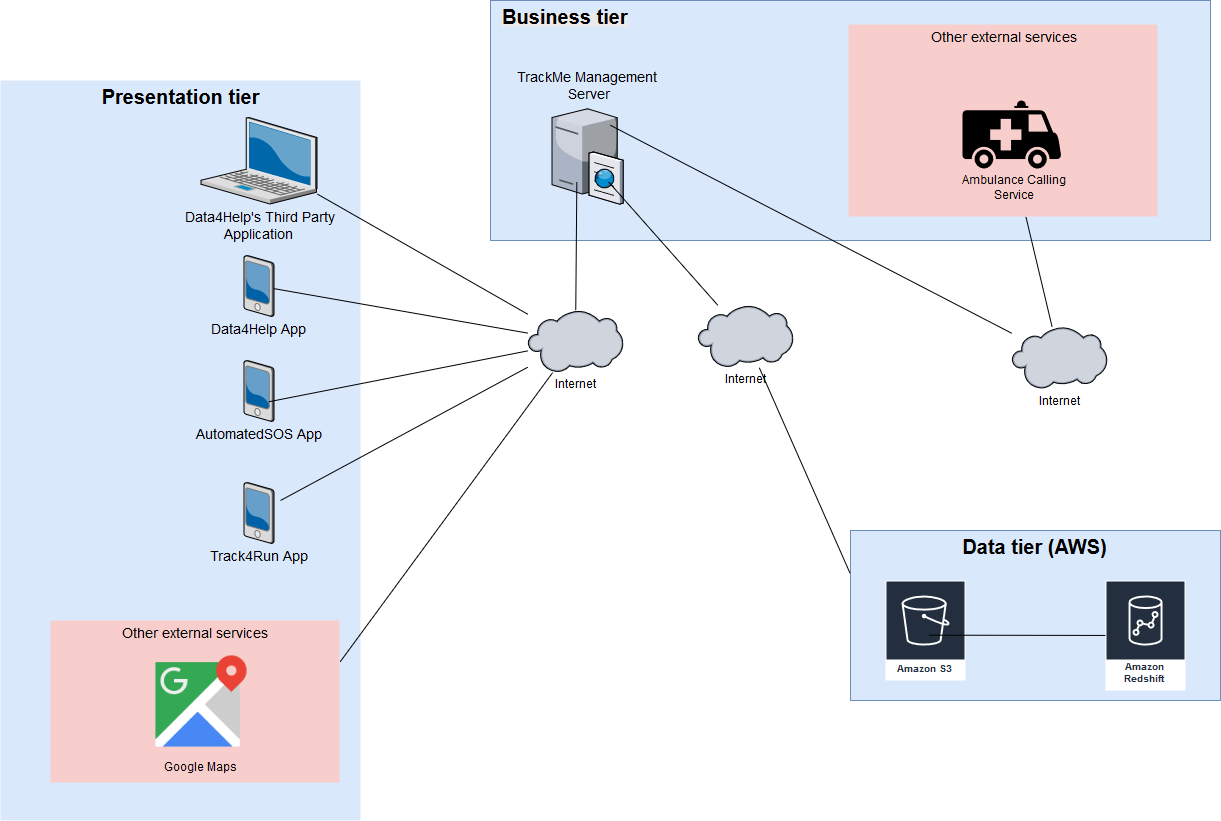
\includegraphics[width=.6\linewidth, height = 20cm, keepaspectratio]{./Images/high_level_architecture_diagram.png}
    \centering
    \caption{High Level Architecture Diagram}
  \end{figure}

\paragraph{Presentation Tier:} is composed by all the client applications, which have only a user interface functionality and do not contain almost any logic. This tier is connected to the Business logic tier.

\paragraph{Business logic tier:} is composed by the server application and the external services excluded AWS, i.e. the hospital calling service. It contains all the core logic of the business, and thus is linked to both the presentation and the data tiers.

\paragraph{Data tier:} is composed by the AWS service. It's function is to provide storage of data used by the logic tier, and hence is linked to it.